\documentclass[a4paper,10pt]{article}
%-----------------------------------------------------------
\usepackage[top=0.75in, bottom=0.75in, left=0.55in, right=0.85in]{geometry}
\usepackage{graphicx}
\usepackage{url}
\usepackage{palatino}
\usepackage{tabularx}
\fontfamily{SansSerif}
\usepackage{hyperref}
\usepackage{fontawesome}

\selectfont

\usepackage[T1]{fontenc}
\usepackage
%[ansinew]
[utf8]
{inputenc}

\usepackage{color}
\definecolor{mygrey}{gray}{0.75}
\textheight=9.75in
\raggedbottom

\setlength{\tabcolsep}{0in}
\newcommand{\isep}{-2 pt}
\newcommand{\lsep}{-0.5cm}
\newcommand{\psep}{-0.6cm}
\renewcommand{\labelitemii}{$\circ$}

\pagestyle{empty}
%-----------------------------------------------------------
%Custom commands
\newcommand{\resitem}[1]{\item #1 \vspace{-2pt}}
\newcommand{\resheading}[1]{{\small \colorbox{mygrey}{\begin{minipage}{0.975\textwidth}{\textbf{#1 \vphantom{p\^{E}}}}\end{minipage}}}}
\newcommand{\ressubheading}[3]{
\begin{tabular*}{6.62in}{l @{\extracolsep{\fill}} r}
	\textsc{{\textbf{#1}}} & \textsc{\textit{[#2]}} \\
\end{tabular*}\vspace{-8pt}}
%-----------------------------------------------------------
\makeatletter

\begin{document}
\hspace{0.5cm}\\[-0.2cm]



\textbf{SHIVARAJ K M} \\ 
\indent B - 11, S K LANE, \\
\indent CHIKKAMAVLLI,\\
\indent BANGALORE - 04\\
\indent Email-id :\textbf{sraj03434@gmail.com} \\
\indent Mobile No.: \textbf{9740501518} \\
\indent\faGithub\href{https://github.com/shiva-raj-km}{   shivaraj}\hfill 
\smash{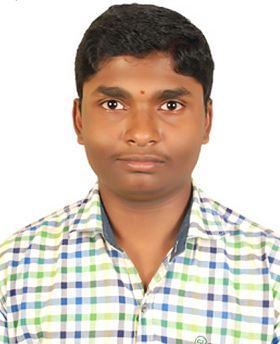
\includegraphics[width=3cm]{1.jpg}}\\

\resheading{\textbf{CAREER SUMMARY} }\\[\lsep]\\ \\
\indent An Electronics and Communication student seeking to pursue a carrier in the field of Robotics,  embedded\\ \indent systems and design.\\

\resheading{\textbf{EDUCATION} }\\[\lsep]
\begin{itemize}
\item \noindent \textbf{Undergraduate (current)}\\
\indent B.E (Electronics and Communication) | BMS College of Engineering, Bangalore | Visvesvaraya Technological University | CGPA 9.42 (5th sem) | Passing Year - 2020.

\item \noindent \textbf{Pre-University}\\
\indent Vijaya Bifr PU College, R V road Bangalore | NCERT (PCME) | Aggregate 89.16\% | Year - 2016.

\item \noindent \textbf{10th SSLC}\\
\indent Bangalore Higher Secondary School, R V road Bangalore | State Board | Aggregate 88.64\% | Year - 2014.
\end{itemize}

\resheading{\textbf{PROJECTS} }\\[\lsep]
\begin{enumerate}
\item\noindent\textbf{ARDOP 3.o(current)}\\
\indent --- Its an Autonomous robot development open source platform. A Humanoid robot capable of doing pick and place of a required object using the vision, kinematics, localization principles. In this project, I am working on vision and power supply management.
\begin{enumerate}
\item\noindent\textbf{Vision}: In vision, object recognition is done using computer neural networks with a darknet53 archeitecture and method used is YOLO(you only look once).
\item\noindent\textbf{Power supply} A power distribution board is build to provide the required power supply to different parts at different power rating.
\end{enumerate}
\item \noindent \textbf{Maze solver robot with Flood fill Algorithm}\\
\indent --- Implemented using Atmega 328 Microcontroller, 8 IR array sensor for line detection. It has two parts dryrun and path tracing:
\begin{enumerate}
\item In dry it covers all the nodes and get the status of each and every node.
\item  After dryrun the algorithm is applied and path tracing starts.
\end{enumerate} 

\item\noindent\textbf{Two wheel Balence Bot}\\
\indent --- A DMP (Digital Motion Processing) algorithm by InvenSense is used for MPU6050 sensor to get the yaw pitch roll values of the current position of the bot. Controller used Atmega 328. A PID cascaded control system is implemented.

\item\noindent\textbf{Gesture Controlled Robot}\\
\indent --- It has two parts transmitter(hand) and reciever(Bot):
\begin{enumerate}
\item  A sensor accelrometer is used in transmitter and based on X and Y value from the sensor direction command is transmitted to bot part.
\item The data received from the transmitter is passed to the controller and command is written to the accuators(motors).
\end{enumerate}
\item\noindent\textbf{MINI projects}\\
1. Smart Parking system using Logic gates.\\
2. Portable Function Generator using MULTISIM simulation software.\\
3. Smart laser locking unit for border security purpose using NodeMCU module.
\end{enumerate}

\resheading{\textbf{INTERNSHIP experience} }\\\\[\lsep]
\begin{itemize}
\item\noindent\textbf{TATA POWER SED Private limited}\\
\indent ---Worked on Electromagnetic Interference and Compatability (EMI and EMC).
\end{itemize}

\resheading{\textbf{TECHNICAL SKILLS} }\\\\[\lsep]
\begin{itemize}
\item \noindent \textbf{Programming Languages}\\
     --\textbf{Proficient:} Embedded C, Python, Verilog\\
     --\textbf{Intermediate:} 8051 Assembly language, Java, MATLAB\\
\item\noindent\textbf{Hardware Knowledge}\\
 8051 microcontroller, Arduino, Atmega 2560, ARM7, Cortex M3, NodeMCU ESP8266, RF and bluetooth modules.\\
\item\noindent\textbf{Software Knowledge}\\
Xilinx Vivado, Cadence Virtuoso, TensorFlow, Matlab and simulink, Multisim, ROS kinetic, Atmel studio, Arduino.
\end{itemize}



\resheading{\textbf{Co-curricular activities} }\\[\lsep]
\begin{enumerate}
\item\noindent \textbf{1\textsuperscript{st} Prize} | National Level Robotics Championship 2018, IIT Kharagpur | Maze solver robot
\item\noindent \textbf{Workshop on App controlled bot} | Conducted workshop on wireless controlled bot by bluetooth communication | BMS College of Engineering
\item\noindent\textbf{Robotics competition} | Perfect Machine | Participated in 2016 NITK Surathkal
\item\noindent\textbf{Huawei Schlarship Award} | For scoring top in ECE department | BMSCE
\end{enumerate}

\resheading{\textbf{Extra curricular activities} }\\[\lsep]
\begin{itemize}
\item \noindent \textbf{Department Volunteer} | Phase Shift 2017 and 2018 | National Level Annual Tech Symposium | BMS College of Engineering
\item \noindent \textbf{Volunteer at Polg Run} | Held on 2\textsuperscript{nd} october 2018 at Bangalore 
\item \noindent \textbf{Publicity Manager at UTSAV 2017} | BMSCE Cultural Event
\end{itemize}

\resheading{\textbf{Personal Details} }\\[\lsep]
\begin{itemize}
\item \noindent \textbf{Father's Name:} MURALIDHAR K S
\item \noindent \textbf{Mother's Name:} MANJULA K M
\item \noindent \textbf{Sex:} Male
\item \noindent \textbf{Date of Birth:} 30 October 1998
\item \noindent \textbf{Nationality:} INDIAN
\item \noindent \textbf{Marital Status:} Single
\end{itemize}


\resheading{\textbf{References} }\\[\lsep]
\begin{itemize}
\item\noindent\textbf{Harish V Mekali}, Assistant Professor, Department of Electronics and Communication, BMSCE, +91 95387 65141, hvm.ece@bmsce.ac.in
\item\noindent\textbf{M N Suma}, Assistant Professor, Department of Electronics and Communication, BMSCE, +91 98866 05910, suma.ece@bmsce.ac.in
\end{itemize}

\resheading{\textbf{Declaration} }\\[\lsep]\\\\
\indent I hereby declare that the above mentioned information is correct to the best of my knowledge and belief\\\\\\
\indent\textbf{DATE:} \@date
\end{document}

